\section{Structures de données}

Stocker le réseau de neurones en mémoire revient à stocker les poids en mémoire, nous devons donc trouver une structure optimale pour stocker ces dernièrs, le temps de calcul n'étant vraiment nécéssaires que lors de la phase du training est peut donc être fait en cloud ou sur un cluster.

L'idée initiale était d'utiliser une matrice tridimensionnelle ayant des dimensions fixes. Mais celà poserai un problème de gachis puisque le nombre des poids différe d'une couche à une autre. Nous avons donc finalement choisi la strucure suivante.

La strucure défini ci-dessous représente l'implémentation de l'exemple en figure 1.

Nous devons noter toute meme que si le nombre des noeuds dans la première couche est $s_0$ le nombre des poids est $(s_0 + 1)s_1$ puisqu'on ajoute le noeud biais (qui n'est pas inclus dans nbNodesLayer1 ni dans le schéma de la figure 1)

\begin{figure}[h]
\centering
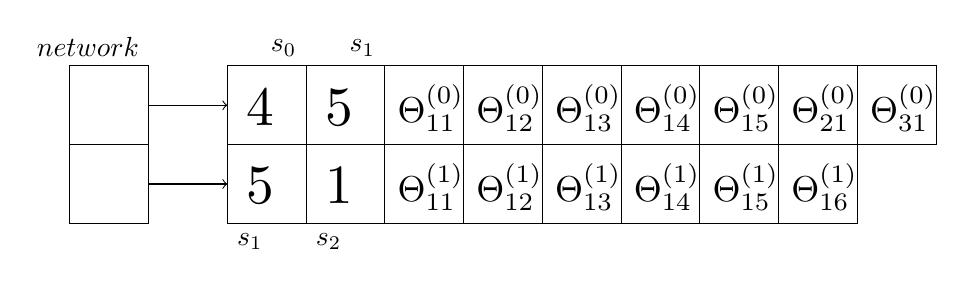
\begin{tikzpicture}

\draw (0, 0)  rectangle (1, 1) node [above left] {$network$};
\draw (0, -1)  rectangle (1, 0);

\draw[->] (1, 0.5) -- (2, 0.5);
\draw[->] (1, -0.5) -- (2, -0.5);

\draw (2, 0)  node [above right, scale=2] {4} rectangle (3, 1) node [above left] {$s_0$};
\draw (3, 0)  node [above right, scale=2] {5} rectangle (4, 1) node [above left] {$s_1$};
\draw (4, 0) node [below right] {} node [above right, scale=1.3] {$\Theta_{11}^{(0)}$} rectangle (5, 1);
\draw (5, 0) node [below right] {} node [above right, scale=1.3] {$\Theta_{12}^{(0)}$} rectangle (6, 1);
\draw (6, 0) node [below right] {} node [above right, scale=1.3] {$\Theta_{13}^{(0)}$} rectangle (7, 1);
\draw (7, 0) node [below right] {} node [above right, scale=1.3] {$\Theta_{14}^{(0)}$} rectangle (8, 1);
\draw (8, 0) node [below right] {} node [above right, scale=1.3] {$\Theta_{15}^{(0)}$} rectangle (9, 1);
\draw (9, 0) node [below right] {} node [above right, scale=1.3] {$\Theta_{21}^{(0)}$} rectangle (10, 1);
\draw (10, 0) node [below right] {} node [above right, scale=1.3] {$\Theta_{31}^{(0)}$} rectangle (11, 1);

\draw (2, -1) node [below right] {$s_1$} node [above right, scale=2] {5} rectangle (3, 0);
\draw (3, -1) node [below right] {$s_2$} node [above right, scale=2] {1} rectangle (4, 0);
\draw (4, -1) node [below right] {} node [above right, scale=1.3] {$\Theta_{11}^{(1)}$} rectangle (5, 0);
\draw (5, -1) node [below right] {} node [above right, scale=1.3] {$\Theta_{12}^{(1)}$} rectangle (6, 0);
\draw (6, -1) node [below right] {} node [above right, scale=1.3] {$\Theta_{13}^{(1)}$} rectangle (7, 0);
\draw (7, -1) node [below right] {} node [above right, scale=1.3] {$\Theta_{14}^{(1)}$} rectangle (8, 0);
\draw (8, -1) node [below right] {} node [above right, scale=1.3] {$\Theta_{15}^{(1)}$} rectangle (9, 0);
\draw (9, -1) node [below right] {} node [above right, scale=1.3] {$\Theta_{16}^{(1)}$} rectangle (10, 0);

\end{tikzpicture}
\caption{Structure de donnée utilisé}
\end{figure}

Pour le moment les poids ne sont représenté que par un tableau statique, nous envisageons de changer celà, en effet Dlib offre un support assez complet des matrices, nous pourrons utiliser le type \textit{matrix<double, 0, 1>}.
Qui améliorera de facon significative la lisibilité et la perfermance du code (cf. Plus loin).
